  
%%%%%%%%%%%%%%%%%%%%%%%%%%%%%%%%%%%%%%%%%

% LaTeX Template for IAHR YPN Congress

%%%%%%%%%%%%%%%%%%%%%%%%%%%%%%%%%%%%%%%%%

%----------------------------------------------------------------------------------------
%	PACKAGES AND OTHER DOCUMENT CONFIGURATIONS
%----------------------------------------------------------------------------------------

\documentclass[landscape,a0paper,fontscale=0.245]{baposter} % Adjust the font scale/size here

\usepackage{graphicx} % Required for including images
\graphicspath{{figures/}} % Directory in which figures are stored

\usepackage{hyperref}
\hypersetup{colorlinks, citecolor=blue, filecolor=blue, linkcolor=blue, urlcolor=blue}

\usepackage{amsmath} % For typesetting math
\usepackage{amssymb} % Adds new symbols to be used in math mode
\DeclareMathOperator*{\argmax}{arg\,max}

\usepackage{booktabs} % Top and bottom rules for tables
\usepackage{enumitem} % Used to reduce itemize/enumerate spacing
\usepackage{palatino} % Use the Palatino font
\usepackage[font=small,labelfont=bf]{caption} % Required for specifying captions to tables and figures

\usepackage{multicol} % Required for multiple columns
\setlength{\columnsep}{1.5em} % Slightly increase the space between columns
\setlength{\columnseprule}{0mm} % No horizontal rule between columns

\usepackage{tikz} % Required for flow chart
\usetikzlibrary{shapes,arrows} % Tikz libraries required for the flow chart in the template

\newcommand{\compresslist}{ % Define a command to reduce spacing within itemize/enumerate environments, this is used right after \begin{itemize} or \begin{enumerate}
\setlength{\itemsep}{1pt}
\setlength{\parskip}{0pt}
\setlength{\parsep}{0pt}
}

\definecolor{lightblue}{rgb}{0.145,0.6666,1} % Defines the color used for content box headers

\begin{document}

\begin{poster}
{
headerborder=closed, % Adds a border around the header of content boxes
colspacing=1em, % Column spacing
bgColorOne=white, % Background color for the gradient on the left side of the poster
bgColorTwo=white, % Background color for the gradient on the right side of the poster
borderColor=lightblue, % Border color
headerColorOne=black, % Background color for the header in the content boxes (left side)
headerColorTwo=lightblue, % Background color for the header in the content boxes (right side)
headerFontColor=white, % Text color for the header text in the content boxes
boxColorOne=white, % Background color of the content boxes
textborder=roundedleft, % Format of the border around content boxes, can be: none, bars, coils, triangles, rectangle, rounded, roundedsmall, roundedright or faded
eyecatcher=true, % Set to false for ignoring the left logo in the title and move the title left
headerheight=0.14\textheight, % Height of the header
headershape=roundedright, % Specify the rounded corner in the content box headers, can be: rectangle, small-rounded, roundedright, roundedleft or rounded
headerfont=\Large\bf\textsc, % Large, bold and sans serif font in the headers of content boxes
%textfont={\setlength{\parindent}{1.5em}}, % Uncomment for paragraph indentation
linewidth=2pt % Width of the border lines around content boxes
}
%----------------------------------------------------------------------------------------
%	TITLE SECTION 
%----------------------------------------------------------------------------------------
%
{
\includegraphics[height=6em]{Seaver_logo.jpeg}} % First university/lab logo on the left
{\bf\textsc{Evaluating Treatment Options for Chronic Kidney Disease Stage 5 using a Markov Decision Process}\vspace{0.5em}} % Poster title
{\textsc{Brian Bowers}} % Author names and institution
{
\includegraphics[height=6em]{school_logo.png}} % Second university/lab logo on the right


%----------------------------------------------------------------------------------------
%	ABSTRACT
%----------------------------------------------------------------------------------------

\headerbox{Abstract}{name=abstract,column=0,row=0}{

Chronic Kidney Disease (CKD) affects approximately 1 in 7 U.S. adults \([5]\), many of whom remain unaware of their condition. The disease progresses gradually, ultimately reaching a stage in which the kidneys lose their ability to effectively filter waste and excess fluid from the bloodstream. A Markov Decision Process (MDP) can be used to model the progression of CKD, providing insight into the disease's impact and helping identify optimal treatment strategies over time.
\vspace{0.6em}

\vspace{0.3em} % When there are two boxes, some whitespace may need to be added if the one on the right has more content
}

%----------------------------------------------------------------------------------------
%	Background
%----------------------------------------------------------------------------------------

\headerbox{Background}{name=introduction,column=1,row=0}{

CKD progresses through five distinct stages, each indicating a greater loss of kidney function. The following terms are necessary to understand this project:    
\begin{itemize}\compresslist
    \item Quality of Life (QoL): ranges from 0.0 to 1.0 
    \item Quality Adjusted Life Years (QALY)
    \item Dialysis: Catheter vs Fistula
    \item Conservative Care (CC): not transplant or dialysis
\end{itemize}

}

%----------------------------------------------------------------------------------------
%	Method 1
%----------------------------------------------------------------------------------------

\headerbox{Method 1}{name=results,column=1, below=introduction}{

\textbf{Value Iteration}: The MDP we have has an infinite horizon (not a fixed time), so the optimal policy is stationary (depends only on the current state). The model will always end in a terminal state.  We use additive rewards where the discount factor, \(\gamma=1\). Utilities are defined based on the QoL. To get the expected utility:
\begin{equation*}
    U^{\pi}_s = E[\sum_{t = 0}^{\infty} \gamma^t R(S_t)]
\end{equation*}    
To get the optimal policy:
      
\begin{equation*}
    \pi^*_s = \argmax_\pi U^{\pi} (s)
\end{equation*}
Then use the Bellman equation to iteratively get the next transition:

\small
\begin{equation*}
    U_{t+1}(s) \leftarrow R(s) + \gamma \max_{a \in A(s)} \sum_{s'} P(s' \mid s, a)U_i(s')
\end{equation*}

Keep applying the updates until the greatest change is lower than some \(\epsilon\).
}


    %----------------------------------------------------------------------------------------
    %	Value Iteration Results
    %----------------------------------------------------------------------------------------
    
    \headerbox{Value Iteration Results}{name=method,column=2, span=2, bottomaligned=results}{ % This block's bottom aligns with the bottom of the conclusion block
    \begin{center}
        \begin{tabular}{l l l l l l}
        \toprule
        \textbf{Metric} & \textbf{Cumulative Rewards} & \textbf{Normalized} & \textbf{Adjusted} \\
        \midrule
        \textbf{Dialysis} & 29.62 & 0.442 & 0.392 \\
        \textbf{CC} & 8.75 & 0.130 & 0.116 \\
        \textbf{Transplant} & 67.04 & 1.000 & 0.887 \\
        \textbf{Fistula} & 29.62 & 0.442 & 0.392 \\
        \textbf{Dialysis w/ fistula} & 25.84 & 0.385 & 0.342 \\
        \end{tabular}
    \end{center}

    The first column is the cumulative rewards, the second is normalized to one, and the third is normalized to the transplant value from method 2. The best policy is to choose transplant, and if you are in dialysis choose fistula.

    \vspace{1em}

    \noindent
    \begin{minipage}{0.65\linewidth}
        \centering
        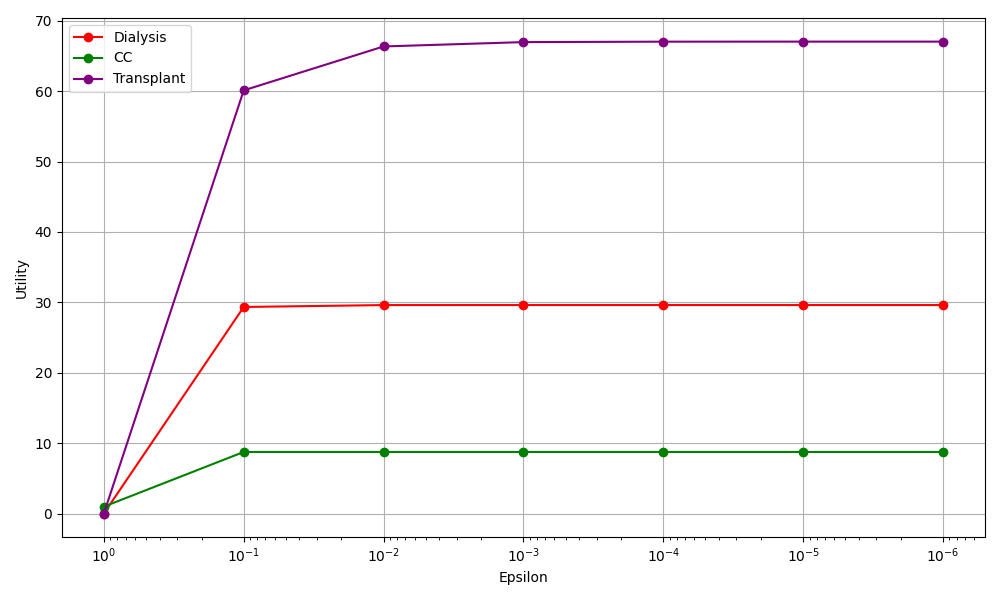
\includegraphics[width=0.9\linewidth]{e_vs_util.png}\\
        \scriptsize Utility vs Epsilon

        \vspace{1em}

        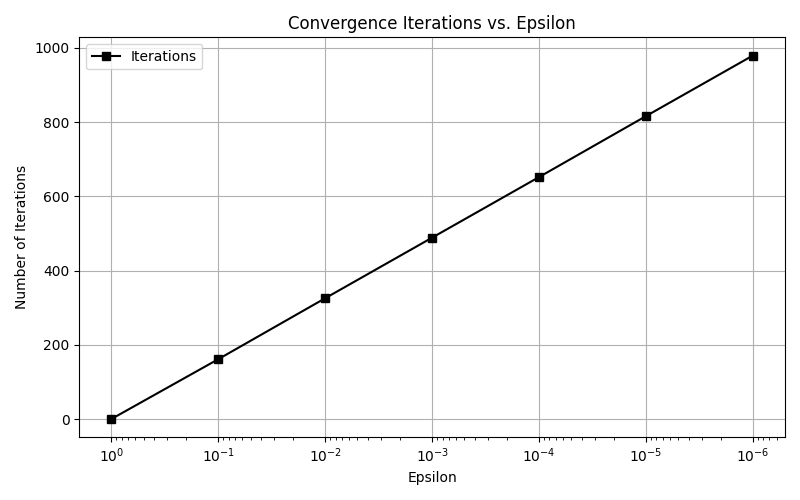
\includegraphics[width=0.9\linewidth]{e_vs_iters_1.png}\\
        \scriptsize Iterations vs Epsilon
    \end{minipage}
    \hfill
    \begin{minipage}{0.35\linewidth}
        \setlength{\rightskip}{2em}

        The plot on the left shows that the utility values converge at low values of epsilon. This means that the epsilon value of \(10E-4\) was small enough to result in accurate results. \\ \\

        \vspace{{4em}}

        The second plot shows the utility and the number of iterations it takes for the MDP to converge. Interesting, there is a linear relationship between the two.
    \end{minipage}
}


%----------------------------------------------------------------------------------------
%	Model
%----------------------------------------------------------------------------------------

\headerbox{Model}{name=method,column=0,below=abstract, bottomaligned=results}{

This model assumes that a patient is currently in CKD stage 5. We use a Markov Decision Process (MDP) to model the disease.

\begin{itemize}\compresslist
\item \(s_0\): the initial state
\item ACTION(\(s\)): a set of actions in each state
\item \(P(s' | s, a)\): transition model
\item \(R(s)\): reward function
\item \(\pi\): solution, which is a policy
\end{itemize}

In our model, \(s_0\) is CKD stage 5, and the patient must decide on a treatment. The options are conservative care (CC), transplant, or dialysis.

Regardless of the choice of treatment, there are several conditions that the patient is at risk for, including stroke, stroke leading to disability, myocardial infarction (MI), MI leading to congestive heart failure, and death.
}



%----------------------------------------------------------------------------------------

\end{poster}

%///////////////////////////////////////////////////////////////////
%///////////////////////////////////////////////////////////////////
%///////////////////////////////////////////////////////////////////
%///////////////////////////////////////////////////////////////////
%///////////////////////////////////////////////////////////////////
%///////////////////////////////////////////////////////////////////
%///////////////////////////////////////////////////////////////////

\clearpage
\begin{poster}
    {
    headerborder=closed, % Adds a border around the header of content boxes
    colspacing=1em, % Column spacing
    bgColorOne=white, % Background color for the gradient on the left side of the poster
    bgColorTwo=white, % Background color for the gradient on the right side of the poster
    borderColor=lightblue, % Border color
    headerColorOne=black, % Background color for the header in the content boxes (left side)
    headerColorTwo=lightblue, % Background color for the header in the content boxes (right side)
    headerFontColor=white, % Text color for the header text in the content boxes
    boxColorOne=white, % Background color of the content boxes
    textborder=roundedleft, % Format of the border around content boxes, can be: none, bars, coils, triangles, rectangle, rounded, roundedsmall, roundedright or faded
    eyecatcher=true, % Set to false for ignoring the left logo in the title and move the title left
    headerheight=0.14\textheight, % Height of the header
    headershape=roundedright, % Specify the rounded corner in the content box headers, can be: rectangle, small-rounded, roundedright, roundedleft or rounded
    headerfont=\Large\bf\textsc, % Large, bold and sans serif font in the headers of content boxes
    %textfont={\setlength{\parindent}{1.5em}}, % Uncomment for paragraph indentation
    linewidth=2pt % Width of the border lines around content boxes
    }
    %----------------------------------------------------------------------------------------
    %	TITLE SECTION 
    %----------------------------------------------------------------------------------------
    %
    {
\includegraphics[height=6em]{Seaver_logo.jpeg}} % First university/lab logo on the left
    {\bf\textsc{Evaluating Treatment Options for Chronic Kidney Disease Stage 5 using a Markov Decision Process}\vspace{0.5em}} % Poster title
    {\textsc{Brian Bowers}} % Author names and institution
    {
\includegraphics[height=6em]{school_logo.png}} % Second university/lab logo on the right
    
    %----------------------------------------------------------------------------------------
    %	Method 2
    %----------------------------------------------------------------------------------------

    \headerbox{Method 2}{name=results2,column=0}{ % This block's bottom aligns with the bottom of the conclusion block

    We can also solve the MDP through simulation. Start in \(s_0\), which is CKD stage 5, and from there, we apply the transition by taking a random weighted choice to get to the next state. If we reach a decision node then we randomly make the choice. This approach allows for more analysis such as the number of months each patient lives after being diagnosed with CKD 5, the average QoL, and the average QALY.
    }
    

    %----------------------------------------------------------------------------------------
    %	REFERENCES
    %----------------------------------------------------------------------------------------
    
    \headerbox{References}{name=references,column=0, below=results2}{
    
    \renewcommand{\section}[2]{\vskip 0.05em} % Get rid of the default "References" section title
    \nocite{*} % Insert publications even if they are not cited in the poster
    \small{ % Reduce the font size in this block
    \bibliographystyle{unsrt}
    \bibliography{sample} % Use sample.bib as the bibliography file
    }}
    
    
    %----------------------------------------------------------------------------------------
    %	SIMULATION RESULTS
    %----------------------------------------------------------------------------------------
    
    \headerbox{Simulation Results}{name=conclusion,column=1,span=3}{
        \begin{center}
            \begin{tabular}{l l l l l l}
            \toprule
            \textbf{Decision} & \textbf{Months (Mean)} & \textbf{Months (SD)} & \textbf{QoL (Mean)} & \textbf{QoL (SD)} & \textbf{QALY}\\
            \midrule
            CC & 10.164369 & 9.566915 & 0.726293 & 0.272583 & 0.615192 \\
            Dialysis, Fistula & 50.832281 & 50.297105 & 0.774744 & 0.130685 & 3.281833 \\
            Dialysis, OneMonth & 45.413938 & 45.875516 & 0.707516 & 0.170910 & 2.677592 \\
            Transplant & 109.760794 & 112.305906 & 0.887768 & 0.162923 & 8.120172 \\
            Transplant, Fistula & 162.093939 & 122.189669 & 0.897094 & 0.035479 & 12.117785 \\
            Transplant, OneMonth & 156.330637 & 118.209652 & 0.882115 & 0.047723 & 11.491801 \\
            \bottomrule
            \end{tabular}
            \captionof{table}{Results from simulation with 100,000  Note: OneMonth means regular dialysis with no fistula}
        \end{center}
    
        \noindent
            \begin{minipage}{0.60\linewidth}
            \centering
            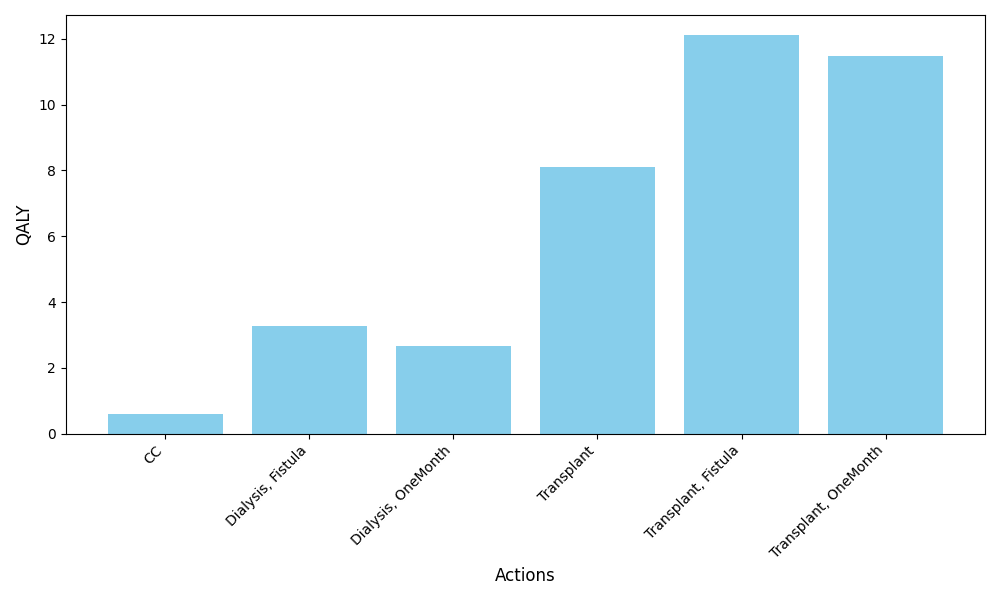
\includegraphics[width=0.65\linewidth]{actions_vs_qaly.png}\\
            \scriptsize QALY values for Different Actions
            
            \vspace{1em}
            
            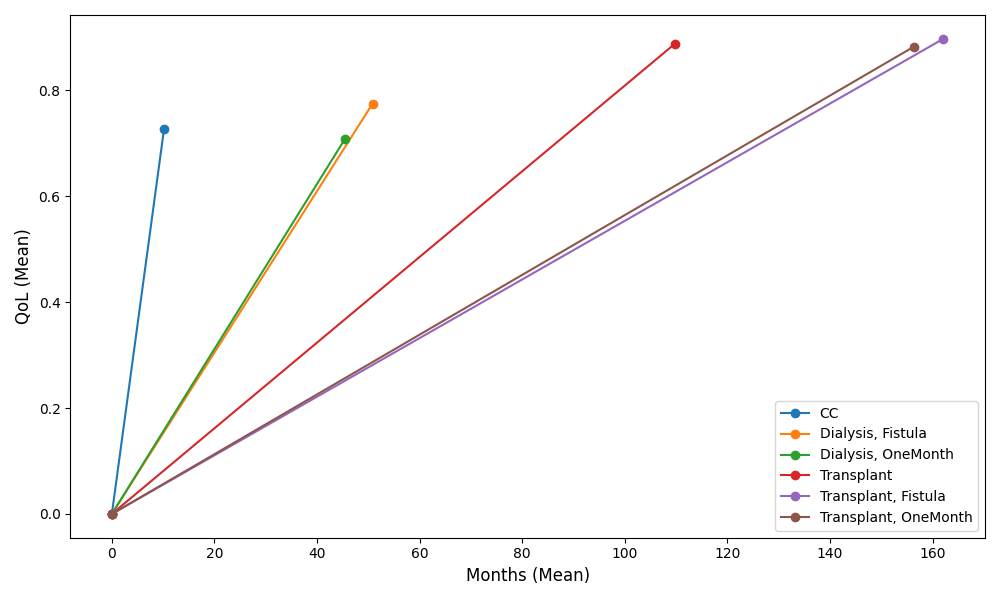
\includegraphics[width=0.65\linewidth]{months_vs_qol.png}\\
            \scriptsize QoL vs Months for Different Actions
            \end{minipage}
            \hfill
            \begin{minipage}{0.40\linewidth}
            \setlength{\rightskip}{6em}

            The graph on the right clearly shows that the most QALY is from transplant, and then fistula. This means that if you have a transplant, and then it fails, you should then go onto dialysis with a fistula. People who outlive their transplant are rare, so it makes sense they would live longer if they outlive their transplant and then go on dialysis. Therefore, our results match with method 1, you should choose transplant, and if you need dialysis you should choose fistula.
            \\
            The second graph shows QoL vs the lifespan of an individual. This is just another way to represent QALY. It is interesting how the CC has a fairly high QoL, but a very short lifespan, resulting in its low QALY. The model seems to reward living longer, but some patients may prioritize short-term QoL over the long-term QALY. If we wanted to model this, we could add in a discount rate, similar to the \(\gamma\) value in method 1, which may alter our results slightly, depending on the value of \(\gamma\). \\
        \end{minipage}



    }


    
    \end{poster}

\end{document}